% ----------------------------------------------------------------
% AMS-LaTeX Paper ************************************************
% **** -----------------------------------------------------------
\documentclass{amsart}
\usepackage{graphicx}
\usepackage{tikz}
% ----------------------------------------------------------------
\vfuzz2pt % Don't report over-full v-boxes if over-edge is small
\hfuzz2pt % Don't report over-full h-boxes if over-edge is small
% THEOREMS -------------------------------------------------------
\newtheorem{thm}{Theorem}[section]
\newtheorem{cor}[thm]{Corollary}
\newtheorem{lem}[thm]{Lemma}
\newtheorem{prop}[thm]{Proposition}
\theoremstyle{definition}
\newtheorem{defn}[thm]{Definition}
\theoremstyle{remark}
\newtheorem{rem}[thm]{Remark}
\numberwithin{equation}{section}
% MATH -----------------------------------------------------------
\newcommand{\norm}[1]{\left\Vert#1\right\Vert}
\newcommand{\abs}[1]{\left\vert#1\right\vert}
\newcommand{\set}[1]{\left\{#1\right\}}
\newcommand{\Real}{\mathbb R}
\newcommand{\eps}{\varepsilon}
\newcommand{\To}{\longrightarrow}
\newcommand{\BX}{\mathbf{B}(X)}
\newcommand{\A}{\mathcal{A}}
% ----------------------------------------------------------------
\begin{document}

\title{MAD 6306 Complex Networks  - Spring 2024\\{\bf Homework 1}}%
\author{Instructor: Jia Liu}%
\date{}

%\dedicatory{}%
%\commby{}%
% ----------------------------------------------------------------

\maketitle
% ----------------------------------------------------------------
\begin{itemize}
\item DUE on 002/02/2025 11:59pm C.T.
\item You can write on the separate work sheet or type your quiz. ( Word or Latex or similar)
\item If you use the handwriting, Solutions must be neat,clear and legible.
\item If you need to scan you quiz, save it as a PDF file. Do not use jpeg, png, jpg etc. Do not submit more than one file.
\item Please check your scanned file before submission. Make sure it is readable, correct order, properly oriented. Make sure it does include all pages.
\item Please name your file as follows: $LastnameInitials-MAD6306hw1.pdf$.If your name is Alan David Roberts, file name is $RobertsAD-MAD6306hw1.pdf$.
\item Try to keep the file size less than 4MB.
\item You can resubmit the quiz if you want. Please specify which one is the one to be graded. Otherwise I will grade the most recent version.
\item DO NOT EMAIL me the quiz. All quizzes are submitted via Canvas.
\end{itemize}


\clearpage
\begin{enumerate}

%---------------------------------------------------------------------------------
% ##############################################################################
% Problem 1
% ##############################################################################
\item Consider the following adjacency matrix of a network
\begin{equation*}
{A}  = \left\lbrack\begin{array}{ccccc}
0 & 0 & 1 & 1 & 0 \\
1 & 0 & 0 & 0 & 0 \\
0 & 1 & 0 & 1 & 0 \\
0 & 0 & 0 & 0 & 0 \\
1 & 0 & 1 & 0 & 0 \\
\end{array}\right\rbrack
\end{equation*}

\begin{enumerate}
\item Is the network directed or undirected? (Explain why).
\item Draw the network.
\end{enumerate}

\vspace{1cm}

\textbf{ \larger[3]Solution} 
\vspace{0.5cm}
\begin{enumerate}
% #######################
% Problem 1-a
% #######################
    \item The nework is directed because the adjacency matrix is asymmetric.
$ A \neq A^T$
\vspace{1cm}
% #######################
% Problem 1-b
% #######################
    \item Network
    
    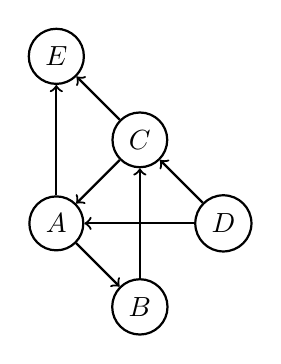
\begin{tikzpicture}[node distance={15mm}, thick, main/.style = {draw, circle}] 
        \node[main] (1) {$A$}; 
        \node[main] (2) [below right of=1] {$B$}; 
        \node[main] (3) [above right of=1] {$C$}; 
        \node[main] (4) [above right of=2] {$D$}; 
        \node[main] (5) [above left of=3] {$E$};
        \draw[->] (1) -- (2); 
        \draw[->] (3) -- (1);  
        \draw[->] (4) -- (1); 
        \draw[->] (1) -- (5); 
        \draw[->] (3) -- (5); 
        \draw[->] (4) -- (3); 
        \draw[->] (2) -- (3); 
    \end{tikzpicture}

\end{enumerate}

\vspace{1cm}

\clearpage
% ##############################################################################
% Problem 2
% ##############################################################################
\item Given the set of node V with $|V | = 6$ in which each node i is labelled by
a natural number between 1 and 6,$ i = 1, 2, 3, 4, 5, 6$, consider the directed
network$ G = (V, E)$ where each link from node j to node i indicates that
j is a multiple of i.
\begin{enumerate}
\item Draw the network.
\item Write down the adjacency matrix of the network.
\end{enumerate}

\vspace{0.5cm}
\textbf{ \larger[3]Solution} 
\vspace{0.5cm}

\begin{enumerate}
% #######################
% Problem 2-a
% #######################
    \item network
    
    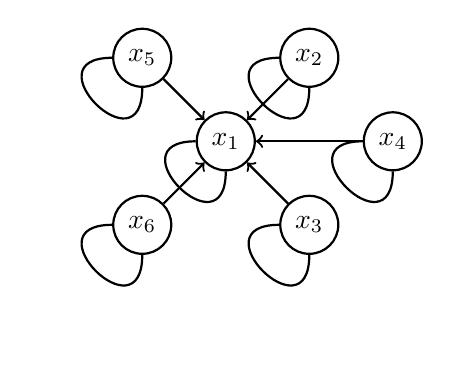
\begin{tikzpicture}[node distance={15mm}, thick, main/.style = {draw, circle}] 
        \node[main] (1) {$x_1$}; 
        \node[main] (2) [above right of=1] {$x_2$}; 
        \node[main] (3) [below right of=1] {$x_3$}; 
        \node[main] (4) [above right of=3] {$x_4$}; 
        \node[main] (5) [above left of=1] {$x_5$}; 
        \node[main] (6) [below left of=1] {$x_6$}; 
        \draw (1) to [out=180,in=270,looseness=5] (1); 
        \draw[<-] (1) -- (2);
        \draw[<-] (1) -- (3); 
        \draw[<-] (1) -- (4); 
        \draw[<-] (1) -- (5); 
        \draw[<-] (1) -- (6);  
        \draw (2) to [out=180,in=270,looseness=5] (2); 
        \draw (3) to [out=180,in=270,looseness=5] (3);
        \draw (4) to [out=180,in=270,looseness=5] (4);
        \draw (5) to [out=180,in=270,looseness=5] (5); 
        \draw (6) to [out=180,in=270,looseness=5] (6); 
    \end{tikzpicture}

\vspace{0.5cm}
% #######################
% Problem 2-b
% #######################
    \item adjacency matrix
    
    \begin{equation*}
        {A}  = \left\lbrack\begin{array}{cccccc}
        1 & 1 & 1 & 1 & 1 & 1 \\
        0 & 1 & 0 & 1 & 0 & 1 \\
        0 & 0 & 1 & 0 & 0 & 1 \\
        0 & 0 & 0 & 1 & 0 & 0 \\
        0 & 0 & 0 & 0 & 1 & 0 \\
        0 & 0 & 0 & 0 & 0 & 1 \\
        \end{array}\right\rbrack
    \end{equation*}
\end{enumerate}

\clearpage

% ##############################################################################
% Problem 3
% ##############################################################################
\item Consider the following two networks: Notwork(a) is directed and Network (b) is undirected but bipartite. Find the following:
\begin{figure}[h]
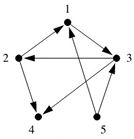
\includegraphics[width=0.2\linewidth]{images/networka.PNG}
\end{figure}

\begin{figure}[h]
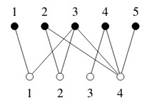
\includegraphics[width=0.2\linewidth]{images/networkb.PNG}
\end{figure}
\begin{enumerate}
\item Find the adjacency matrix of network (a)
\item Find the incidence matrix of network (b)
\end{enumerate}

\vspace{0.5cm}
\textbf{ \larger[3]Solution} 
\vspace{0.5cm}
\begin{enumerate}
    \item Find the adjacency matrix of network (a)
    \begin{equation*}
        {A}  = \left\lbrack\begin{array}{ccccc}
        0 & 1 & 0 & 0 & 1 \\
        0 & 0 & 1 & 0 & 0 \\
        1 & 0 & 0 & 0 & 1 \\
        0 & 1 & 1 & 0 & 0 \\
        0 & 0 & 0 & 0 & 0 \\
        \end{array}\right\rbrack
    \end{equation*}
    \item Find the incidence matrix of network (b)
    \begin{equation*}
        {A}  = \left\lbrack\begin{array}{cccc}
        1 & 0 & 0 & 0 \\
        0 & 1 & 0 & 1 \\
        1 & 1 & 0 & 1 \\
        0 & 0 & 1 & 1 \\
        0 & 0 & 0 & 1 \\
        \end{array}\right\rbrack
    \end{equation*}
\end{enumerate}
\vspace{5cm}

\clearpage
% ##############################################################################
% Problem 4
% ##############################################################################
\item Which word or words from the following list describe each of the five networks below: {\em directed, undirected, cyclic, acyclic, approximately acyclic, planar, approximately planar, tree, approximate tree}.
\begin{enumerate}
\item The internet, at the level of autonomous systems
\item A food web
\item The stem and branches of a plant
\item A spider web
\item A complete clique of four nodes
\end{enumerate}

\vspace{0.5cm}
\textbf{ \larger[3]Solution} 
\vspace{0.5cm}

\begin{enumerate}
    \item The internet, at the level of autonomous systems
    
        Undirected, Acyclic, Approximately planar 
        \vspace{0.5cm}
    \item A food web
        
        Directed, Cyclic 
        \vspace{0.5cm}
    \item The stem and branches of a plant
        
        Tree, Acyclic 
        \vspace{0.5cm}
    \item A spider web
        
        Undirected, Planar 
        \vspace{0.5cm}
    \item A complete clique of four nodes
        
        Undirected, Cyclic 
        \vspace{0.5cm}
\end{enumerate}
\vspace{5cm}
\clearpage
% ##############################################################################
% Problem 5
% ##############################################################################
\item A simple network consists of n nodes in a single component. What is the maximum possible number of edges it could have? What is the minimum possible number of edges it could have? 

\vspace{0.5cm}
\textbf{ \larger[3]Solution} 
\vspace{0.5cm}

By the Handshaking Theorem:

$deg(v_1)+deg(v_2)+deg(v_3)+...+deg(v_n)=2|E|$

G is a simple network  of n nodes in a single component. The maximum possible number of edges is:

$(n-1)+(n-1)+(n-1)+...+(n-1)=2|E|$

$n\left(n-1\right)=2|E|$

$\frac{n\left(n-1\right)}{2}=|E|$
\end{enumerate}

\end{document}
% ----------------------------------------------------------------
